% !TEX encoding = UTF-8
% !TEX TS-program = pdflatex
% !TEX root = ../tesi.tex
% !TEX spellcheck = it-IT

%**************************************************************
\chapter{Framework analizzati}
\label{cap:framework-analizzati}
%**************************************************************
Questo capitolo inizia con una descrizione generale della tipologia di framework analizzati, per poi andare a descrive più in dettaglio il funzionamento dei singoli framewrok, seguito da una sintesi dei pregi e difetti e un breve resoconto riguardo il prototipo realizzato.
Infatti, per valutare al meglio ogni framework è stato realizzata un'applicazione prototipo che visualizza una gallery di immagini ottenuta mediante chiamate ad \gls{API} \gls{REST}.\\
La struttura del prototipo è stata scelta in modo tale da verificare le seguenti caratteristiche:
\begin{itemize}
\item possibilità di disporre le immagini in una griglia;
\item possibilità di implementare lo scroll infinito, una tecnica per ottimizzare il caricamento di grandi quantità di dati che prevede il caricamento iniziale di un limitato numero di elementi, per poi caricare gli elementi rimanenti man mano che l'utente prosegue nella visualizzazione dei dati.
\item fluidità dell'applicazione, specialmente durante il caricamento dei dati;
\item possibilità di personalizzare la barra di navigazione dell'applicazione.
\end{itemize}

\todo[inline]{Valutare se inserire le informazioni riguardo l'esecuzione di un'applicazione}

\section{Considerazioni generali}
Le applicazioni realizzate con questa tipologia di framework hanno alla base lo stesso funzionamento: una \gls{virtual machine} interpreta il codice JavaScript e utilizza un componente ``\textit{ponte}'' per modificare l'interfaccia grafica dell'applicazione, la quale è realizzata con i componenti offerti dal \gls{SDK} nativo.

Ognuno dei framework analizzati utilizza un ``\textit{ponte}'' diverso, il cui funzionamento verrà descritto più in dettaglio nell'apposita sezione.

Un'altra caratteristica di questa tipologia di framework è l'assenza del \gls{DOM}.
Infatti, l'interfaccia di un'applicazione di questo tipo è composta da componenti grafici del sistema operativo che vengono creati e composti a durante l'esecuzione dell'applicazione e non da elementi HTML come nelle applicazioni ibride.

Nel complesso si ottengono due grossi vantaggi:
\begin{itemize}
\item l'esecuzione del codice JavaScript e il \gls{rendering} dell'interfaccia grafica avvengono su due thread distinti, rendendo l'applicazione più fluida;
\item utilizzando i componenti grafici nativi si ottiene un esperienza utente più simile a quella che si ottiene con un'applicazione realizzata in \gls{Obj-C}/Java.
\end{itemize}

\subsection{Differenze con le applicazioni ibride}

Un'applicazione ibrida consiste in un'applicazione nativa composta da una \gls{WebView} che visualizza un'insieme di pagine web realizzate utilizzando HTML5, CSS3 e JavaScript, che replicano l'aspetto di un'applicazione nativa.

Trattandosi quindi di un'applicazione web è possibile utilizzare tutti i framework e le tecnologie disponibili nell'ambito web, come AngularJS o jQuery.

Inoltre, se è già disponibile un'applicazione web per desktop, la creazione di un'applicazione mobile ibrida risulta rapida in quanto è possibile riutilizzare sia parte del codice, sia le competenze legato allo sviluppo web dei vari sviluppatori.

Questo approccio viene utilizzato da qualche anno e permette di creare applicazioni che possono accedere ad alcune funzionalità hardware del dispositivo come il giroscopio o la fotocamera e che possono essere commercializzate nei vari store online.

Per supportare questo processo di sviluppo sono stati sviluppati dei framework come Cordova/\gls{PhoneGap} che si occupano di gestire la WebView e di fornire un sistema di plug-in per accedere alle funzionalità native.

Questa tipologia di applicazioni ha però delle limitazioni riguardanti:
\begin{itemize}
\item \textbf{Prestazioni:} trattandosi di una pagina web renderizzata all'interno di un browser, non è possibile sfruttare al massimo le potenzialità della piattaforma sottostante, come il multi-threading. Questo comporta che il codice JavaScript e il rendering dell'interfaccia grafica vengano eseguiti nello stesso thread, ottenendo così un'interfaccia poco fluida.
\item \textbf{Esperienza d'uso:} una delle caratteristiche principali delle applicazioni native sono le \gls{gesture}, l'utente è abituato ad interagire con le applicazioni native, le quali sono dotate di un complessio sistema di riconoscimento delle gesture che non è ancora replicabile in ambito web.
\item \textbf{Funzionalità:} non tutte le funzionalità che può sfruttare un'applicazione nativa sono disponibili in un'applicazione ibrida.
\end{itemize}

Il funzionamento dei framework analizzati in questo capitolo permette di risolvere i problemi principali delle applicazioni ibride, in quanto sfruttando i componenti nativi, non sono presenti i problemi prestazionali legati al rendering dell'interfaccia grafica, il quale non viene bloccato dall'esecuzione del codice JavaScript. Inoltre, sempre per il fatto che  vengono utilizzati componenti nativi, è possibile sfruttare lo stesso sistema di riconoscimento delle gesture e le stesse animazioni, rendendo l'esperienza d'uso più simile a quella offerta da un'applicazione realizzata con l'SDK nativo.

\section{Tabris.js}

Framework pubblicato da EclipseSource\footnote{\url{http://eclipsesource.com/en/home/}} nel Maggio 2014, che permette di controllare mediante JavaScript i componenti dell'interfaccia grafica nativa, sia di iOS, sia di Android.

\subsection{Come funziona}
Tabris.js funziona utilizzando come "\textit{ponte}" una versione modificata di Cordova, la quale, grazie a dei plug-in sviluppati da EcplipseSoruce, permette di interagire via JavaScript con i componenti nativi del sistema operativo.

Ognuno di questi plug-in incapsula un determinato componente dell'interfaccia grafica e fornisce delle API JavaScript per controllarlo.

Trattandosi di un framework derivato da Cordova è possibile utilizzare i plug-in di Cordova già esistenti per aggiungere nuove funzionalità, oltre  a quelle offerte framework, come per esempio l'utilizzo della fotocamera. 

L'unica condizione per il corretto funzionamento dei plug-in esterni è che non dipendano dal DOM, dal momento che il DOM non è presente durante l'esecuzione di un'applicazione.

Il framework viene pubblicato come open source, tuttavia per accedere al codice sorgente è necessario acquistare una licenza, pertanto non è stato possibile analizzare più in dettaglio il funzionamento del framework.

\subsection{Pregi e difetti}

Uno dei pregi di Tabris.js è quello che il codice JavaScript scritto è indipendente dalla piattaforma, questo permette di utilizzare lo stesso codice sorgente e lo stesso layout sia per iOS sia per Android.
\`E il framework che si occupa di eseguire tutte le operazioni specifiche per le varie piattaforme e di renderizzare gli opportuni componenti grafici.

Un altro pregio deriva dall'estensibilità, è infatti possibile utilizzare sia dei plug-in di Cordova, sia i moduli disponibili su \gls{npm}, con la condizione che questi non dipendano dal DOM.

Le criticità di Tabris.js riguardano per lo più il layout che deve essere fatto in modo imperativo, definendo prima la dimensione e la posizione dei vari componenti, per poi organizzarli in modo gerarchico.

Sempre per quanto riguarda il layout, la personalizzazione è limitata in quanto risulta complesso, se non impossibile, definire dei componenti grafici composti o con layout particolari, come la visualizzazione a griglia.

Infine, il framework non impone né suggerisce alcun pattern architetturale da adottare, lasciando completa libertà al programmatore, con il rischio che il codice sorgente dell'applicazione diventi complesso e difficile da manutenere.

\subsection{Prototipo}

\begin{figure}[htp]
\centering
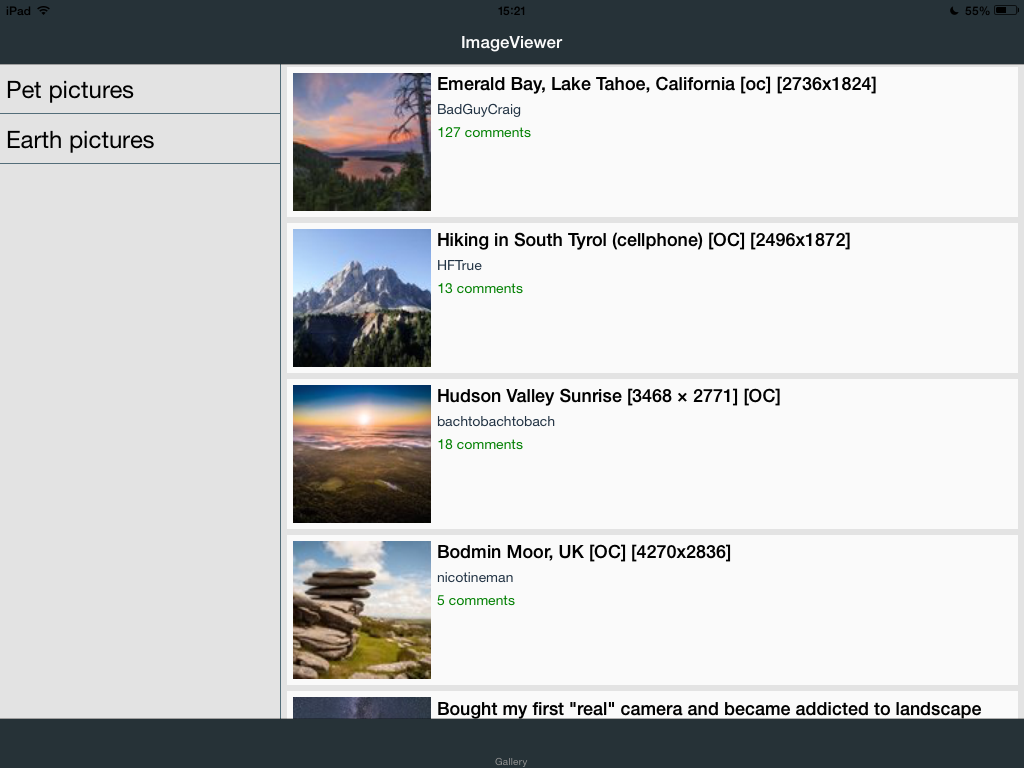
\includegraphics[width=\textwidth]{../immagini/prototipo-tabris}
\caption{Screenshot del prototipo realizzato con Tabris.js}  
\end{figure}

Nel realizzare l'applicazione prototipo sono state riscontrate varie problematiche in particolare riguardanti il layout.
Ad esempio, non è stato possibile disporre gli elementi in una griglia e la personalizzazione della barra di navigazione si è rilevata essere molto limitata.

Un altro problema emerso durante la realizzazione del prototipo è stata la scarsa disponibilità di materiale online, infatti oltre alle risorse messe a disposizione da EclipseSource e alla documentazione ufficiale, non è stato possibile trovare altre informazioni riguardanti il framework.

In ogni caso, l'applicazione realizzata è molto fluida e l'esperienza d'uso è paragonabile a quella di un'applicazione nativa.

\FloatBarrier
\section{NativeScript}

Framework rilasciato da Telerik nel Maggio 2015 che permette di realizzare applicazioni mobile native sia per iOS che per Android rendendo possibile utilizzare tutte le API native mediante JavaScript.

\subsection{Come funziona}

NativeScript utilizza come ``\textit{ponte}'' una virtual machine appositamente modificata che all'occorrenza esegue del codice C++ per invocare le funzioni scritte in linguaggio nativo (Obj-C, Java).

Questa virtual machine deriva da \gls{V8} se l'applicazione viene eseguita su Android o da \gls{JavaScriptCore} nel caso l'applicazione venga eseguita su iOS.

Le modiche subite dalla virtual machine riguardano:
\begin{itemize}
\item la possibilità di intercettare l'esecuzione di una funzione JavaScript ed eseguire in risposta del determinato codice C++;
\item l'iniezione di metadati che descrivono le API native;
\end{itemize} 
In questo modo il runtime di NativeScript può utilizzare i metadati per riconoscere le funzioni JavaScript che hanno una corrispondente funzione nativa, in modo da poter richidere l'esecuzione della funzione nativa mediante del codice C++.

\begin{figure}[htp]
\centering
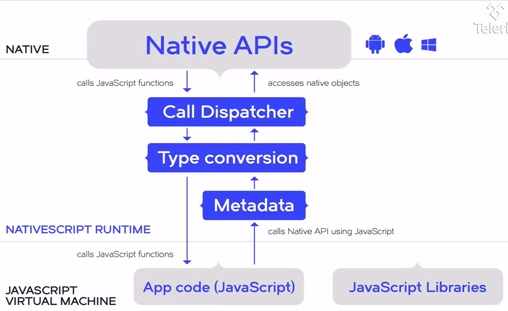
\includegraphics[width=\textwidth*3/4]{../immagini/ns-runtime}
\caption{Schema rappresentante il runtime di NativeScript}  
\end{figure}
\FloatBarrier

Di conseguenza il runtime di NativeScript permette di creare degli oggetti JavaScript che funzionano da \gls{proxy} rispetto agli oggetti nativi specifici della piattaforma.
Un esempio del funzionamento è dato dal seguente codice che su iOS crea un oggetto di tipo \texttt{UIAlertView}:

\begin{lstlisting}[language=JavaScript, caption=Esempio di creazione di un oggetto nativo]
var alert = new UIAlertView();
\end{lstlisting}

All'esecuzione del JavaScript la virtual machine riconosce, grazie ai metadati iniettati, che la funzione JavaScript deve essere eseguita come una funzione nativa.

Di conseguenza, utilizzando del codice C++, invoca la corrispondente funzione Obj-C che in questo caso istanzia un oggetto \texttt{UIAlertView} e memorizza un puntatore all'oggetto nativo in modo da poterlo recuperare in seguito per eseguire delle funzioni su di esso.

Alla fine, la virtual machine crea un oggetto JavaScript che funziona come un proxy dell'oggetto nativo precedentemente creato e lo ritorna in modo che possa essere memorizzato e utilizzato come un normale oggetto JavaScript.

I metadati che vengono iniettati nella virtual machine e che descrivono tutte le funzioni offerte dalle API native della piattaforma, sono ricavati durante il processo di compilazione dell'applicazione utilizzando la proprietà di \gls{riflessione} dei linguaggi di programmazione.

Il vantaggio di questa implementazione è che tutte le API native sono invocabili da JavaScript e anche le future versione delle API potranno essere supportate appena queste vegnono rilasciate.

Inoltre, questi metadati possono essere generati anche per tutte le librerie native di terze parti, rendendole disponibili in JavaScript.

Per permettere il riuso del codice NativeScript fornisce dei moduli che aggiungo un livello di astrazione ulteriore rispetto alle API native, che contiene sia componenti grafici, sia funzionalità comuni ad entrambe le piattaforme, come l'accesso al filesystem o alla rete.
Questo livello di astrazione è opzionale ed è sempre possibile effettuare chiamate dirette alle API native.

\begin{figure}[htp]
\centering
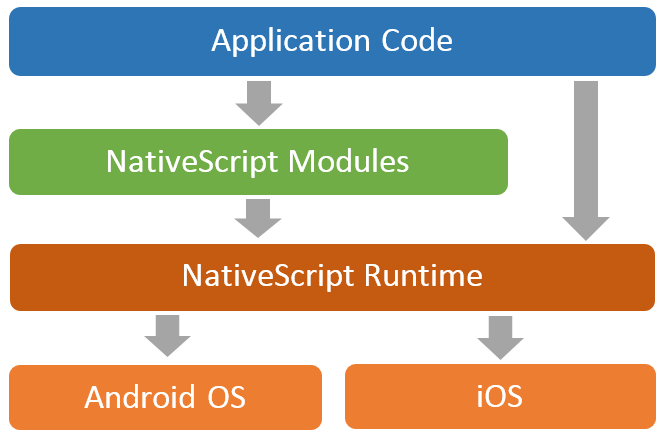
\includegraphics[width=\textwidth/2]{../immagini/ns-architecture}
\caption{Architettura di NativeScript}  
\end{figure}
\FloatBarrier

\subsection{Pregi e difetti}

Il pregio principale di NativeScript è che rende disponibili ad un'applicazione nativa realizzata in JavaScript tutte le funzionalità che possono essere presenti in un'applicazione realizzata con l'SDK nativo. 

Inoltre, l'interfaccia grafica di un'applicazione viene realizzata in modo dichiarativo mediante XML e CSS\footnote{NativeScript implementa un sotto insieme limitato di CSS in quando le istruzioni CSS devono essere applicate sui componenti nativi.}, in un modo analogo a quello utilizzato per le applicazioni web.

Tuttavia, le funzionalità offerte dal livello di astrazione sono limitate e di conseguenza per ottenere effetti particolari è necessario utilizzare le API native.

Questo comporta la diminuzione del codice riusabile su più piattaforme e un notevole aumento della complessità, allontanandosi così dallo scopo principale dell'utilizzo del JavaScript per lo sviluppo di applicazioni native, che è quello di sviluppare in modo semplice e senza utilizzare le API native.

\subsection{Prototipo}

\begin{figure}[htp]
\centering
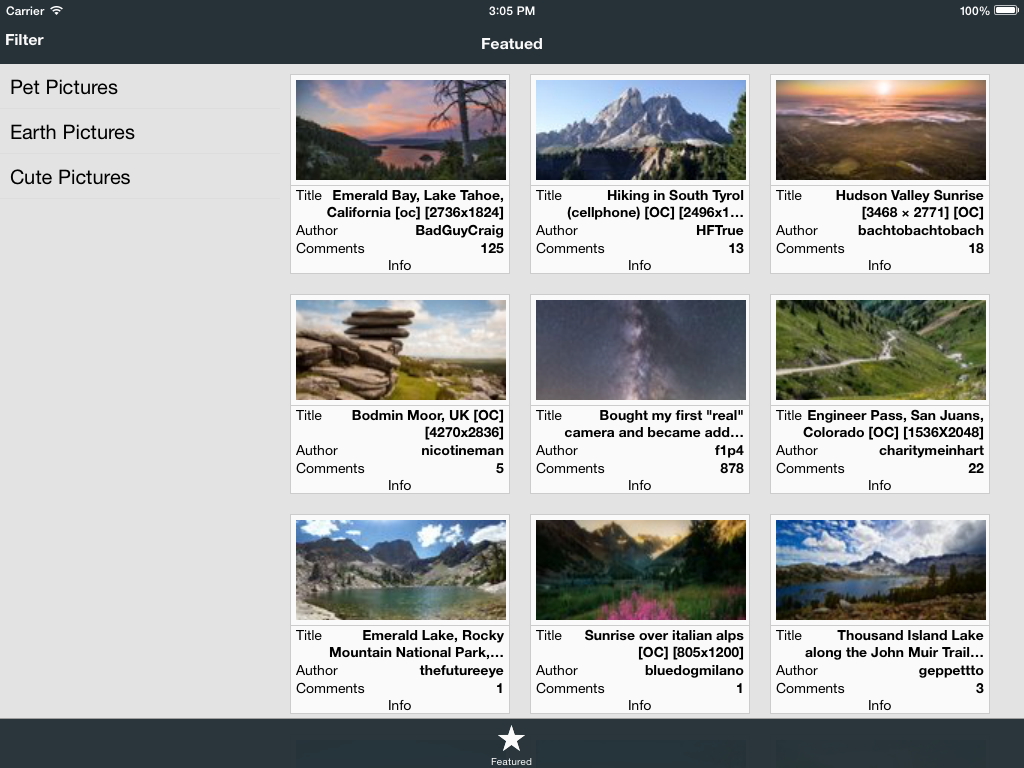
\includegraphics[width=\textwidth]{../immagini/prototipo-react-native}
\caption{Screenshot del prototipo realizzato con NativeScript}  
\end{figure}

Sfruttando quasi solamente i componenti generici offerti da NativeScript è stato possibile ottenere un layout simile a quello dell'applicazione attuale.

Tuttavia per realizzare la visualizzazione a griglia delle immagini è stato necessario utilizzato un componente \texttt{Repeater} all'interno di una \texttt{ScrollView}, questa implementazione risulta poco efficiente e poco fluida, in quanto non essendo mappata su un componente nativo non gode delle stesse ottimizzazioni.

Sono state individuate soluzioni alternative sfruttando librerie native di terze parti, che non sono state adottate in quanto ritenute troppo complesse dal momento che fanno largo uso di codice specifico per iOS.

\FloatBarrier
\section{React Native}

Framework sviluppato da Facebook come progetto interno per la realizzazione di applicazioni native per iOS sfruttando il JavaScript e con un funzionamento analogo a quello di React\footnote{Framework per lo sviluppo di applicazioni web pubblicato da Facebook.}.

React Native è stato successivamente rilasciato come progetto open source nel Marzo 2015.

\subsection{Come funziona}

React Native è composto da una parte scritta in Obj-C e un'altra parte scritta in JavaScript.
La parte realizzata in Obj-C comprende:
\begin{itemize}
\item una serie di classi che definiscono il ``\textit{ponte}'' che permette di alla virtual machine di invocare codice nativo;
\item un'insieme di macro che permettono alle classi Obj-C di esportare dei metodi in modo che questi possano essere invocati dal ``\textit{ponte}'';
\item un'insieme di classi che derivano dai componenti nativi di uso comune e che utilizzano le macro per esportare alcune funzionalità.
\end{itemize}
La parte realizzata in JavaScript consiste in un livello di astrazione, organizzato in moduli, che nascondere l'interazione con le componenti native.

Tra questi moduli si trova la maggior parte dei componenti grafici necessari per la realizzazione di un'interfaccia grafica e per l'accesso ad alcune delle funzionalità del dispositivo, come le notifiche o i servizi di localizzazione. 

\`E inoltre presente il modulo \texttt{NativeModules} che permette di interagire direttamente con il ``\textit{ponte}'' in modo da utilizzare oggetti nativi personalizzati.

Quando viene avvita un'applicazione con React Native, viene eseguito del codice Obj-C che istanzia sia la virtual machine che andrà ad interpretare il JavaScript, sia il ``\textit{ponte}'' tra la virutal machine e il codice nativo.

Durante l'esecuzione del codice JavaScript è possibile richiedere l'esecuzione di codice nativo usando il modulo \texttt{NativeModules}, questo modulo fornisce all'oggetto ``\textit{ponte}'' le informazioni necessarie per permettergli di identificare la porzione di codice nativo da eseguire.
Per poter essere eseguito il codice nativo deve utilizzare le macro fornite da React Native, altrimenti il ``\textit{ponte}'' non riesce ad identificare il metodo da invocare.

Al fine di ottenere prestazioni migliori, la virtual machine che esegue il JavaScript viene eseguita su un thread diverso rispetto a quello che si occupa dell'esecuzione del codice nativo e del rendering dell'interfaccia grafica.

Inoltre, la comunicazione tra questi due thread viene gestita in modo asicrono ed eseguita in blocchi, in questo modo è possibile ridurre le comunicazioni tra i due thread ed evitare che l'interfaccia grafica si blocchi durante l'esecuzione del codice JavaScript.

\subsection{Pregi e difetti}

React Native fornisce un buon livello di astrazione rispetto la piattaforma nativa, dando la possibilità ad uno sviluppatore web di realizzare un'applicazione nativa completa senza conoscere nulla riguardo il funzionamento della piattaforma sotto stante.

A causa di questa astrazione non tutte le funzionalità native sono disponibili, tuttavia è possibile adattare classi Obj-C già esistenti mediante le macro messe a disposizione dal framework, tuttavia questo processo prevede una buona conoscenza del linguaggio Obj-C e della piattaforma sottostante.

Tra gli altri pregi di React Native c'è la community di sviluppatori creatasi attorno al framework, infatti, nonstante si tratti di un framework pubblicato recentemente, si è già creata una community numerosa ed è già possibile trovare dei moduli open source che estendono le funzionalità base del framework.

Infine il flusso di lavoro per lo sviluppo di un'applicazione con React Native risulta molto veloce, in quanto grazie all'utilizzo dei WebSocket, non è necessario eseguire la build dell'applicazione ad ogni modifica del codice sorgente, portando un notevole risparmio di tempo.

\subsection{Prototipo}

\begin{figure}[htp]
\centering
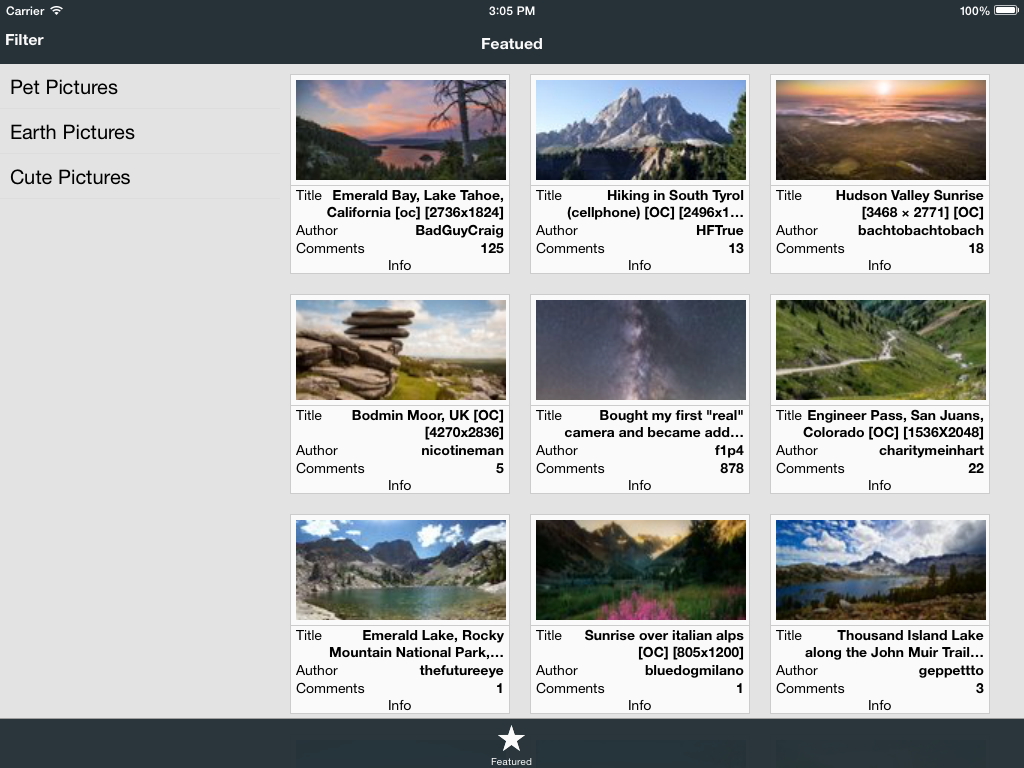
\includegraphics[width=\textwidth]{../immagini/prototipo-react-native}
\caption{Screenshot del prototipo realizzato con React Native}  
\end{figure}

Il prototipo realizzato è stato in grado di soddisfare la maggior parte delle caratteristiche ricercate, infatti è stato possibile ottenere una visualizzazione a griglia, dotata di scroll infinito e fluido.

Sono stati invece incontrati dei problemi riguardanti la personalizzazione della barra di navigazione, in quando il componente offerto dal framework non permette la presenza di pulsanti personalizzati nella barra di navigazione.

Tuttavia sono state individuate alcune soluzioni che prevedono l'utilizzo di moduli open source che forniscono una barra di navigazione maggiormente personalizzabile.

\FloatBarrier
\section{Confronto finale}
\todo[inline]{Trovare un nome migliore}

\begin{table}[h]
\centering

\begin{tabular}{|m{2.3cm}|m{3cm}|m{3cm}|m{3cm}|}
\hline - & Tabris.js & NativeScript & React Native   \\ 
\hline  

Funzionamento & Utilizza dei plug-in di Cordova per rendere accessibili i componenti grafici nativi via JavaScript & Utilizza una VM modificata e dei meta dati relativi alle API native per renderne possibile l'utilizzo via JavaScript  & Utilizza delle classi Obj-C per creare un ponte tra la VM che esegue il JavaScript e le componenti native   \\ 

\hline  

 Possibilità di personalizzazione & Limitata a quanto offerto dal framework & Come se l'applicazione fosse scritta in linguaggio nativo & Limitata a quanto offerto dal framework   \\
 
\hline 

 Estensibilità & Mediante plug-in di Cordova & Mediante librerie native di terze parti & Estendendo librerie native di terze parti con le macro offerte dal framework  \\ 

\hline

 Piattaforme supportate & iOS e Android & iOS e Android & iOS   \\

\hline

\end{tabular}

\caption{Tabella comparativa dei framework analizzati}
\label{my-label}
\end{table}

\FloatBarrier
\section{Framework scelto}

Dopo aver esaminato e confrontato i tre framework individuati si è scelto di utilizzare React Native per la seconda parte dello stage.

Questo perché React Native si è dimostrato un framework molto potente anche se non offre l'accesso completo alle API native come fa NativeScript.
Inoltre, la diffusione già ampia del framework e il supporto da parte di Facebook, che sta attualmente utilizzando React Native per sviluppare alcune delle proprie applicazione, fornisce al framework un'ampia possibilità di crescita, mediante l'estensione di nuove funzionalità o il supporto di ulteriori sistemi operativi, come Android.

Per quanto riguarda NativeScript, è stato scartato principalmente perché non raggiunge l'obiettivo di nascondere la complessità dello sviluppo di un'applicazione nativa con Obj-C o Swift.

Infatti, l'obiettivo che si vuole raggiungere sviluppando un'applicazione nativa in JavaScript è quello di riutilizzare il più possibile le competenze derivate dallo sviluppo web senza dover imparare tutti i dettagli dello sviluppo con l'SDK nativo.

Infine, Tabris.js è stato scartato perché è risultato troppo limitato e non è stato in grado di soddisfare alcune delle caratteristiche ricercate.




